\documentclass[preprint]{elsarticle}

\usepackage{lineno,hyperref}
\modulolinenumbers[5]

\journal{To be determined}
\usepackage{graphicx}
\usepackage{epstopdf}
\usepackage{mathptmx}
\usepackage{amsmath}
\usepackage{amssymb}
\usepackage[linesnumbered]{algorithm2e}
\usepackage{algcompatible}
\usepackage{enumerate}
\usepackage[english]{babel}
\usepackage{multirow}
\usepackage{tabularx}  % for 'tabularx' environment and 'X' column type
\usepackage{ragged2e}  % for '\RaggedRight' macro (allows hyphenation)

%appendix name fix
\usepackage[english]{babel}

%Pretty tables
\usepackage{booktabs}
\setlength\heavyrulewidth{0.2ex}
\setlength\lightrulewidth{0.15ex}
\setlength\cmidrulewidth{0.15ex}

\usepackage{caption}
\usepackage[utf8]{inputenc}
\usepackage{subcaption}

%for drawing over the notation table
\usepackage{tikz}

%set double spacing
\usepackage{setspace}

%Allow more figures per page
\renewcommand{\floatpagefraction}{.999}


%%%%%%%%%%%% FIX SECTIONS LATEXDIFF %%%%%%%%%%%%%%%%%%%%%
\usepackage{xcolor}
\DeclareRobustCommand{\hsout}[1]{\texorpdfstring{\sout{#1}}{#1}}
\DeclareRobustCommand{\hwave}[1]{\texorpdfstring{\uwave{#1}}{#1}}
\RequirePackage[normalem]{ulem}% DIF PREAMBLE
\RequirePackage{color}\definecolor{DELETIONS}{rgb}{1.0,0.0,0.0}
\RequirePackage{color}\definecolor{ADDITIONS}{rgb}{0.0,0.6,0.0}
\providecommand{\DIFadd}[1]{{\protect\textcolor{ADDITIONS}{\hwave{#1}}}}% DIF PREAMBLE
\providecommand{\DIFdel}[1]{{\protect\textcolor{DELETIONS}{\hsout{#1}}}}% DIF PREAMBLE
%\providecommand{\DIFdel}[1]{{\protect}}% DIF PREAMBLE

%%%%%%%%%%%%%%%%%%%%%%%%%%%%%%%%%%%%%%%%%%%%%%%%%%%%%%%%%%%%%%%

\usepackage{verbatim}

\begin{document}

\title{Improving recommendation of useful pieces of information for users to better understand current context}

\begin{spacing}{2}

\begin{frontmatter}

\author[addressjorge,addressjie]{Jorge Castro\corref{mycorrespondingauthor}}
\ead{jcastro@decsai.ugr.es}

\author[addressjie]{-Jie Lu}
\ead{jie.lu@uts.edu.au}

\author[addressjie]{-Guangquan Zhang}
\ead{guangquan.zhang@uts.edu.au}

\author[addressluis]{Luis Mart\'inez}
\cortext[mycorrespondingauthor]{Corresponding author}
\ead{martin@ujaen.es}

\address[addressjorge]{Department of Computer Science and Artificial Intelligence, University of Granada, Granada (Spain)}
\address[addressjie]{School of Software, University of Technology Sydney, Sydney (Australia)}
\address[addressluis]{Computer Science Department, University of Ja\'en, Ja\'en (Spain)}

\begin{abstract}

Recommender systems (GRSs) filter relevant items to users in overloaded search spaces using information about their preferences. In this scenario, there are succesful RSs for several domains including recommendation of news and QA, among others. The traditional recommendation scheme consists of analysing the terms used in the item to generate an item profile and a user profile that later is used to recommend items that match user profiles. This basic scheme can be further improved considering that context influences user preferences. Some examples of contexts are the device where the recommendations are shown, companion of the target user or trends in current interest according to what others talk about. In the latter case, there have been . This paper focuses on the context extracted from the latter scenario, in which a feed of status updates of a well-known social network is used. When the information is extracted in such a way, there are several key aspects in the context integration with the user profile, such as context cleaning, aggregation and weighting. This paper explores such aspects and proposes a recommender system that integrates context to improve QA recommendation with context information. A case study will evaluate the results on several datasets, showing that the context integration benefits recommendation.

\begin{keyword}
   \texttt{recommender systems} \sep \texttt{context-aware recommendation} \sep \texttt{user profile contextualisation}
\end{keyword}
\end{abstract}

\end{frontmatter}

\section{Introduction}\label{sec:introduction}

%Information overload and Recommender Systems
Users satisfaction in current scenario is affected by the amount of information available. This situation originates that users need to put a significant effort for finding relevant pieces of information for them. In some scenarios it might not be possible for users to explore information items in order to select the most suitable one. The \emph{information overload} problem impacts users satisfaction. Recommender Systems have been a powerful tool for alleviating information overload in large search spaces. RSs have been proven to be successful in several domains, such as e-health \cite{}, \cite{}. In this paper we focus on QA recommendation with contextual information integration.

%RSs approaches
There are several approaches within RecommenderSystems. The most widespread ones are Collaborative Filtering (CFRS) and Content Based (CBRS). The main difference among them is that CFRS focuses on user preferences, while CBRS focuses on the analysis on items descriptions. Therefore, the performance of these recommendation approaches is subject to the quality and amount of available information.

%CBRSs
Within CBRSs we distinguish two kinds of CBRSs: (i) based on item features, (ii) based on items descriptions. In this paper we focus on the latter, given that QA items have a strong component of textual information for both explaining the question and answering it. Although CBRSs need some input from user preferences (user cold-start) and suffer from overfitting (lack of diversity in recommendations) \cite{}, CBRS have demonstrated their utility when new items are introduced in the system, i.e., item cold-start \cite{Aggarwal2016}. This feature makes it interesting to apply CBRS approaches in domains where new items are constantly introduced, such as web pages or news. In this direction, QA recommendation share the features that make it interesting to apply CBRSs, hence, we focus on them.

%Boundary of knowledge in QA recommendation with CBRSs.
In this scenario there are several proposals for QA recommendation with CBRS approaches. 




%Parrafo de contexto: Explicación de por qué introducimos basado en contexto.
Justification of context-aware recommendation.


%Boundary of knowledge of QA recommendation with contextual information:



\section{Preliminaries}

This section provides the required background for the current research, including basics about CBRS, and related works in content based recommendation with context awareness.

\subsection{Content-based recommender systems.}

An accurate definition of Recommender System (RS) given by R. Burke \cite{Burke2002} is \emph{"any system that produces individualized recommendations as output or has the effect of guiding the user in a personalized way to interesting or useful objects in a large space of possible options"}. Within RSs, various techniques can be distinguished. 

Hablar de mi paper de IJIS.

TfIdf.

LSA sobre TfIdf.

Hibridacion con colaborativos, \cite{Symeonidis2007} 

Otras basadas en contenido

\subsubsection{CBRSs relacionados con la propuesta}

EnTagRec \cite{Wang2014} is not a CBRS, but it works on keywords. An Enhanced Tag Recommendation System for Software Information Sites. Individual user recommender system to retrieve tags for a new post that is evaluated in several STS: Stack Overflow, Ask Ubuntu, Ask Different, and Free code. Offline evaluation with Precision@10 and Recall@10.

\cite{Shao2017} Recommending Answerers for Stack Overflow with LDA Model. Recommends unanswered questions to users to encourage faster answers. Matches topic of the question with the expertise of the target user. Offline evaluation on StackOverflow dump. Accuracy as evaluation measure.

\cite{Odiete2017} Recommending Programming Languages by Identifying Skill Gaps Using Analysis of Experts. A Study of Stack Overflow. Helps developers expand their knowledge by suggesting them to learn the programming language that fits his/her expertise gaps using expertise graphs.

\cite{Lipczak2010} Learning in efficient tag recommendation. Tag recommendation system. It does not propose a new algorithm, but a way to update the model in order to incorporate new information to it without needing to build it from scratch. It does offline evaluation with DelicioUs dataset and Stack Overflow. Precision and recall are used as evaluation measures.

\cite{Zheng2015b} A Hybrid Trust-Based Recommender System for Online Communities of Practice. It is a recommender system to find answerers to a specific question formulated by an asker. This RS uses the hybrid trust network of the asker and combines content analysis to extract the keywords of the question. They achieve higher precision and recall. They perform offline experimentation to detect whether the


\subsection{Context-aware recommender systems.}

Traditional recommender systems can be classified on six classes based on the knowledge source \cite{DePessemier2016}: demographic recommendations, knowledge-based
recommendations, community-based recommendations, content-based recommendations,
collaborative recommendations, and hybrid recommendations. As noted by R.Burke \cite{Burke2002} other sources of information can be considered in the recommendation, such as the context in which the recommendation is received by users, and F. Ricci \cite{Ricci2012contextualizing} stated that the conditions or circumstances in which the recommendation is delivered significantly affect the decision behaviour of the users. Therefore, the consideration of users' context is key to provide interesting recommendations.

With this regard, the various context-aware recommendation approaches can be classified into three classes \cite{Adomavicius2011}:
\begin{itemize}
	\item Pre-filtering: The system selects the feedback gathered in the same context in which the recommendation is delivered to the user.
	\item Post-filtering: The recommendations are generated first without considering contextual information. After that, the item predictions are modified regarding the specific context of the users, possibly filtering out some items.
	\item Contextual modelling: The contextual information is directly integrated in the model that is used to recommend.
\end{itemize}

In Contextual Pre-filtering, the approach is to filter out the information that was not not gathered in the current context. With this regard, in traditional RSs the information is viewed as a function $R: User \times Item \rightarrow Rating $ that the RS tries to approximate. In CARS, the information can be viewed as a three dimensional cube $User \times Item \times Context \rightarrow Rating$. Contextual pre-filtering selects only the information relative to the context, hence, it tries to approximate function $R_{context}: User \times Item \rightarrow Ratings_{context}$ This way, they only consider ratings generated in the context in which the recommendation is delivered to the user. Contextual pre-filtering is a simple and effective approach, but it is affected by data sparsity when there is not enough information generated in all contexts to provide accurate recommendations. Some researchers have tried to overcome this issue through context-generalization \cite{Adomavicius2011}, that generalizes the context when the information available in the current context is not enough and includes information from the broader context.

In contextual post-filtering, the recommendations are first computed overlooking the contextual information, as in traditional RSs. After this initial step, recommendations are tuned to adjust to the current context \cite{Panniello2009}, either removing irrelevant items or through a weighting function that changes predictions of items regarding the suitability of target user's context. A previous work \cite{} evaluated them in the same scenarios and compared pre- and post-filtering approaches. It determined that neither pre-filtering nor post-filtering completely dominates the other and a study to determine the best approach is needed in each specific case.

Previous approaches try to reduce the CARS problem to a two dimensional one that can be solved with traditional RSs. This is not the case in contextual modelling, in which contextual information is directly incorporated in the recommendation model to recommend. With this regard, researchers have explored heuristic-based \cite{Panniello2014}, probabilistic \cite{Adomavicius2005b}, or matrix factorization \cite{Baltrunas2011c} contextual modelling approaches.

\subsubsection{CA-CBRSs relacionacos con este trabajo}

\cite{Ponzanelli2014} Libra: RS for supporting programmers complete issues and bugs using query completion. They perform online testing assessing the percent of success of a programmer that is using Libra with a control group.

\cite{Ponzanelli2017} Harnessing stack overflow for the IDE. Presents a plug-in for eclipse that enables stack overflow searches contextualized to the language and other relevant. It does no evaluation whatsoever.

\cite{Ponzanelli2014b} Prompter: A Self-Confident Recommender System. The same as the previous one. Proposes a plug-in that automatically searches on stack overflow. This one notifies the user if it is confident enough of the answer provided. The user can provide the confidence level that has to be reached to trigger “proactive” help.

\cite{Parikh2009} Buzz-based recommender system. This system looks somewhat similar to the system that we want to develop, but on eCommerce. This one is based on buzzwords used in the text input of the search within eBay. Our work will be based on buzzwords detected on twitter to recommend historic questions on StackExchange (Any site).

\cite{DePessemier2016} This paper does A user-centric evaluation of context-aware recommendations for a mobile news service. Hace una evaluación de un Sistema de recomendación basado en contenido con información contextual. Es interesante para tenerlo en cuenta como técnica a comparar


\subsection{Related works in context-aware content-based recommender systems.}



\section{Proposal}

The proposal is composed of several parts:
11
\begin{enumerate}
	\item Extract information of the QA domain.
	\begin{itemize}
		\item TfIdf
		\item LSA over TfIdf
	\end{itemize}
	\item Building user preference profile: Aggregate 
	\item Context profile building
	\item Contextualization of user profiles
	\item Prediction
\end{enumerate}


\section{Extract information of the QA domain.}

In the QA dataset there is textual information of the question and its related answers. In this proposal we treat all the i

\subsection{TfIdf}

In this proposal we consider posts as the document, and the words used in their text as the terms. The terms are stemmed using the Porter Stemmer algorithm \citep{Porter1980}. Once stemmed, their term frequency is computed using the raw count of appearance on the document:
\begin{equation}
	profile_{d} = \{tf_{t,d}~~~~s.t.~~~~ t \in d \} ~~~~,  ~~~~~~
	tf_{t,d} = f_{t,d}
\end{equation}

Once the term frequency is computed for all terms in all documents, the inverse document frequency is calculated for each term.

\begin{equation}
	idf_t = - \log( N / n_t )
\end{equation}

Finally, the values of the profiles are weighted with the $idf_t$ of each term:
\begin{equation}
	profile_d = \{w_{t,d} ~~~~s.t. ~~~~t\in d\} ~~~~,  ~~~~~~
	w_{t,d} = tf_{t,d}*idf_t
\end{equation}

\subsection{LSA over TfIdf}

Once the tf-idf profiles are built, LSA is performed to reduce the dimensionality of the matrix. LSA is proven to be effective through the description of both document and words in a reduced number of features, while reducing the negative impact of synonyms in the text \cite{}. Therefore, the aim of this step is to decompose the word-document in: word-features matrix ($U$), singular value vector ($s$), and document-features matrix ($V$):

\begin{equation}
	TFIDF_{(|D|\times|T|)} = U_{(|D|\times k)} * s_{(k)} * V'_{(k \times |W|)}
\end{equation}

The proposal performs an approximated factorisation of the TF-IDF matrix using singular value decomposition, which allows to reduce the dimensionality of the original matrix keeping the $k$ most relevant singular values of the original matrix.

Hence, we obtain the profile of both terms and documents in the reduced space:
\begin{equation}
	profile_d = \{ U_{t,1},\dots, U_{t,k}\}
\end{equation}

\begin{equation}
	profile_t = \{ V_{t,1},\dots, V_{t,k}\}
\end{equation}

\section{Building user preference profile: Aggregate words' profiles}

At this point the proposal has built a model to describe documents and words. In order to provide personalised recommendation to users, it is needed to build user profiles in the same space. The information the system holds about users is a unary matrix that states whether the user has expressed interest in the document either by creating, commenting, or voting it:

\begin{table}
	\caption{Users' preferences over items, the rating matrix.}
	\label{tab:user-preferences}
	\centerline{\small\baselineskip=13pt
	\begin{tabular}{|c||ccccc|}
		\hline
         &     $i_1$     & $\dots$  &     $i_k$     & $\dots$  & $i_n$
		\tabularnewline
		\hline
		\hline
$u_1$    & $r_{u_1,i_1}$ & $\dots$  & $r_{u_1,i_k}$ & $\dots$  & $r_{u_1,i_n}$
		\tabularnewline
$\vdots$ & $\vdots$      & $\ddots$ & $\vdots$      & $\ddots$ & $\vdots$
		\tabularnewline
$u_j$    & $r_{u_j,i_1}$ & $\dots$  & $r_{u_j,i_k}$ & $\dots$  & $r_{u_j,i_n}$
		\tabularnewline
$\vdots$ & $\vdots$      & $\ddots$ & $\vdots$      & $\ddots$ & $\vdots$
		\tabularnewline
$u_m$    & $r_{u_m,i_1}$ & $\dots$  & $r_{u_m,i_k}$ & $\dots$  & $r_{u_m,i_n}$
		\tabularnewline
		\hline
	\end{tabular}}
\end{table}

With this table we can get the set of documents that user $u$ has expressed interest in:
\begin{equation}
	R_{u} = {d ~~~~s.t.~~~~r_{u,d} =1 }
\end{equation}

This way, the user profile is built upon the profiles of the documents that belong to $R_u$:

\begin{equation}
	profile_u = \sum_{d \in R_u} V_d = \{ \sum_{d \in R_u} V_{d,1}, \dots, \sum_{d \in R_u} V_{d,k}\}
\end{equation}

This user profile describes the user preferences in terms of the singular values.

\section{Context profile building}

In parallel with the building of the user profile, it is needed to build the context profile. In this proposal we assume that the source of the context is a microblogging system that delivers status updates by users. To narrow down the status updates that the system receives in order to focus in an aspect of the context. Therefore, there is a set of terms that must appear in the status updates.

First, from al the terms that the context contains, the proposal filters out the terms that do not appear in the set of terms used in the QA site. 

Given that the context is composed of several status updates, there can be a mixing of topics. In order to separate the topics of the context and select the most suitable one, the proposal performs a fuzzy clustering of the words of the context. Hence, the fuzzy c-means clustering algorithm groups the terms using the feature vector of the words as the word definition.

Once the terms of the context are grouped, the proposal generates a context profile for each cluster. A profile of each cluster is generated combining the profiles of the words that are included in each of them.

Based on the terms that appear on the context we can build the profile of the context using the feature representation of each term from the QA domain.

\begin{equation}
	profile_{T_c} = \{\sum_{t \in T_c} U_{t,1}, \dots, \sum_{t \in T_c} U_{t,k} \}
\end{equation}

\section{Contextualization of user profiles}

Once we have the user profile and the context profile, it is needed to combine them in order to provide personalised recommendation that are suited to the current context $T_c$:

\begin{equation}
	profile_u^{T_c} = \alpha * profile_u + (1- \alpha )*profile_{T_c}
\end{equation}

\begin{equation}
	profile_u^{T_c} = \{ \alpha * profile_{u,1} + (1- \alpha ) * profile_{T_c,1},\dots, \alpha * profile_{u,1} + ( 1 - \alpha ) * profile_{T_c,k} \}
\end{equation}

\section{Prediction}

Once we have the contextualised user profile, we can produce a prediction of the suitability for a given item regarding the profile:
\begin{equation}
	p_{u,d} = profile_u^{T_c}*s*profile_d
\end{equation}

The recommendation is a list of documents sorted by $p_{u,d}$.

\section{Experiment}

To evaluate the proposal, we performed an experiment that simulates the recommendation of QA items in in various context. The remainder of the section is structured as follows. First, the settings of the experiment are described. The datasets and methods for processing are then detailed. After that, the evaluation measures are commented. Lastly, the results are analysed.

\subsection{Experimental procedure}

In these experiments, a RS based on LSA modelling with contextual information is evaluated (LSAContext). The baseline method to compare with is the LSA method without contextual information. 30 features are considered in LSA and LSAContext models.

In order to do the experiment, the following procedure is performed \cite{Sarwar2001}, with a modification to consider contextual information in the experiment:
\begin{itemize}
	\item Split the dataset in training and test.
	\item Build the model with the training data.
	\item Build the profile of each user. Include contextual information.
	\item Recommend to each user based on their profile and the model.
	\item Evaluate recommendations with the test set.
\end{itemize}

This procedure is repeated 20 times and 5-cross fold validation is used to split the data in training and test sets. Moreover, various contexts are considered, which are detailed in the following section.

\subsection{Methods compared}

We compared several recommendation techniques to integrate contextual information in QA recommendation. Here, we show the results of three ways of characterise the context:

\begin{itemize}

	\item No clustering: The words are not separated in clusters, therefore the context profile is unique. There is a single profile of the context that is built combining the profiles of the words that are included in the context.
	\begin{equation}
		profile_{T_c} = \sum_{t \in T_c} * profile_t
	\end{equation}

	\item Max membership: The words are used only in the cluster to whom they have the highest membership value:
	\begin{equation}
		profile_{cluster_l} = \sum_{t \in T} \mu^{max}_{t,l} * profile_t
	\end{equation}

	\item Weithed by membership: The cluster profiles are built combining the feature vector of each word weighted by the membership value of the word to the cluster:
	\begin{equation}
		profile_{cluster_l} = \sum_{t \in T} \mu_{t,l} * profile_t
	\end{equation}
	\noindent where $\mu_{t,l}$ is the membership of term $t$ to cluster $l$.

\end{itemize}

Moreover, the proposals compared have parameter $\alpha$. In the experiment we explored several values for it, here, to make the results clear, we show the results for $\alpha \in [0.85,1.00]$ with increments of $0.01$

\subsection{Datasets}

In the experiment there are two sources of data: The QA domain and the contextual information.

The QA domain used is the StackExchange dataset\footnote{http://data.stackexchange.com/}. This dataset consists of the database dump of each site in the stackexchange ecosystem. Some sites are detailed in Table \ref{tab:stackexchange-dataset-description}, together with their main features.

In this experimental setup, the results are reported per StackExchange site. Therefore, we consider each site as a different dataset. Given that the aim of the system is to provide users with pieces of information that help explain the context and also consider their preferences.

Regarding the contextual dataset, a set of interesting keywords is defined. We have selected the terms \emph{news}, \emph{current} and \emph{situation}. From these seed terms, we extracted a dataset of tweets that contain any of these words from twitter. The stats of the dataset extracted is depicted in Figure \ref{fig:context-dataset-description}.

\begin{figure}[htb]
    \centering
    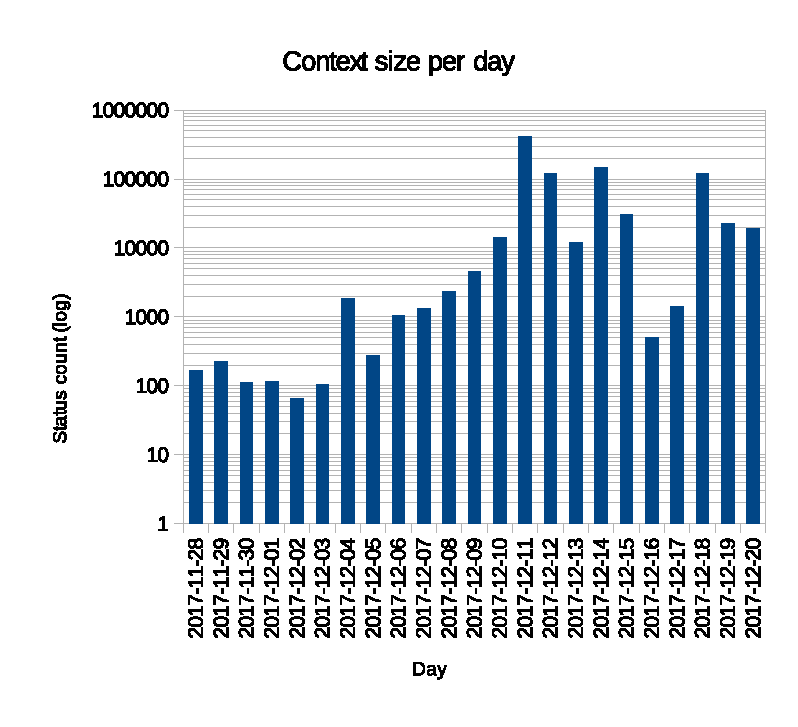
\includegraphics[width=0.5\textwidth]{figures/context-dataset-description.eps}
    \caption{Contextual dataset used in the experiment, where each day has a different status count.}
    \label{fig:context-dataset-description}
\end{figure}

\subsection{Evaluation Measures}

Usually, measures to evaluate the prediction errors in terms of rating deviation are used. However, the methods being compared do not provide a rating prediction, but a value that expresses the suitability of items regarding the user profile. Therefore, the measures that can be used are information retrieval ones, such as precision and recall. Researchers have remarked that, although they are useful, they are not sensible to the sorting of the items that the RSs does \cite{Gunawardana2015}. In order to consider the quality of the sorting, the NDCG is used:

\begin{equation}
	DCG_u = \sum_{k=1}^N\frac{r_{u,recom_{u,k}}}{log_2 (k+1)}
\end{equation}

\noindent where $recom_{u,k} \in I$ is the item recommended to user $u$ in $k$ position.

\begin{equation}
	NDCG = \frac{DCG}{DCG_{perfect}}
\end{equation}

\noindent where $DCG_{perfect}$ is a perfect sorting of the items, i.e., the list of items sorted by their value in the test set.

\subsection{Results}

In this section, the results obtained for the different approaches compared are shown and analysed to evaluate the performance of the proposal.

Table \ref{tab:results-ndcg-3dprinting} shows the results of the compared approaches in the 3dprinting site.

\begin{figure}[htb]
    \centering
    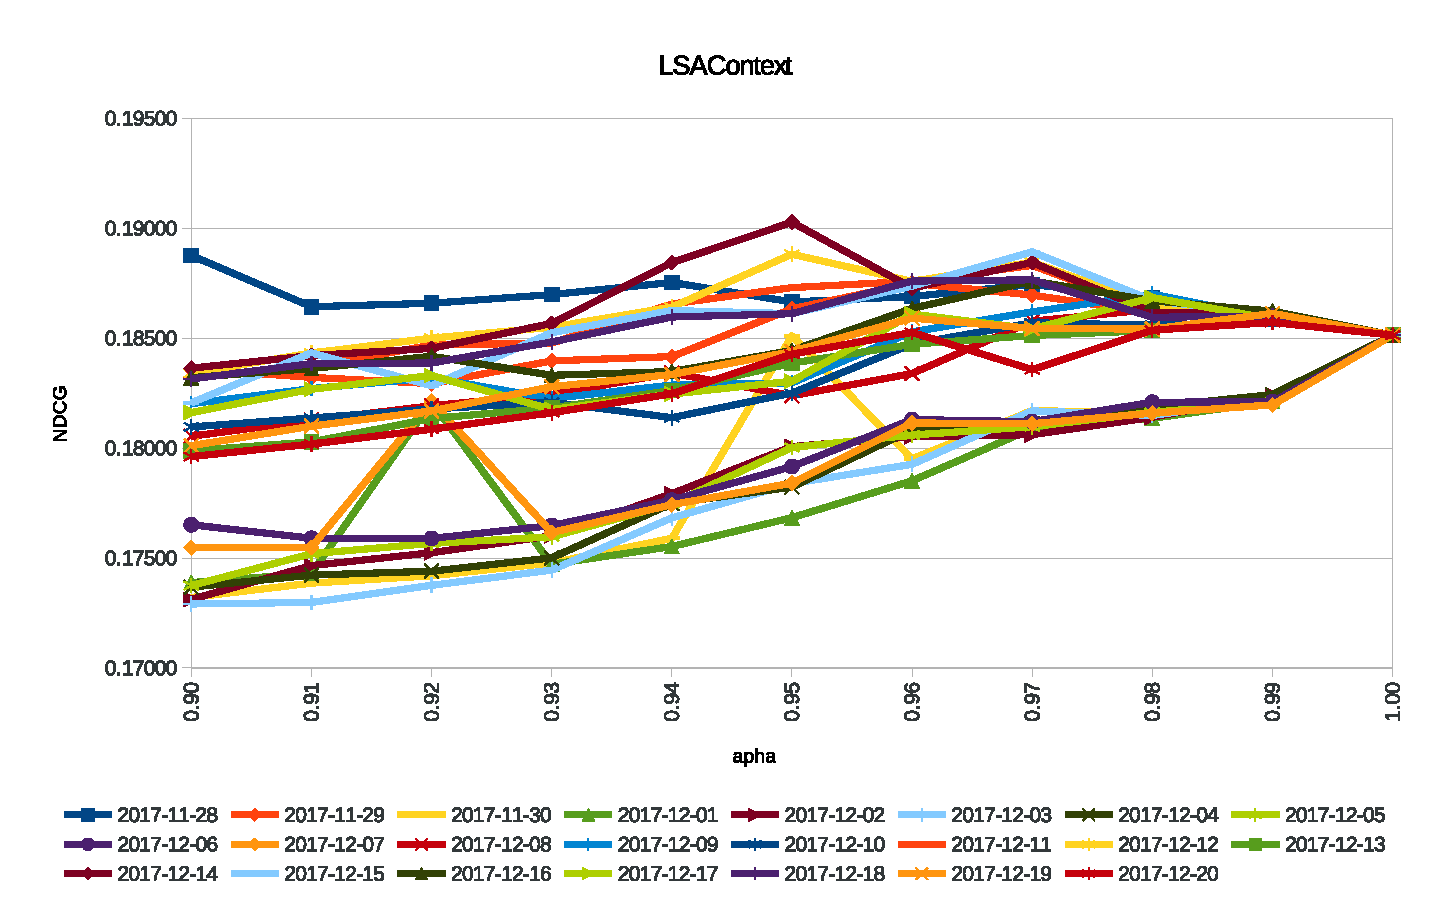
\includegraphics[width=0.33\textwidth]{figures/ndcg-results-proposal-context-no-clustering.eps}
    \caption{Contextual dataset used in the experiment, where each day has a different status count.}
    \label{fig:ndcg-results-proposal-context-no-clustering}
    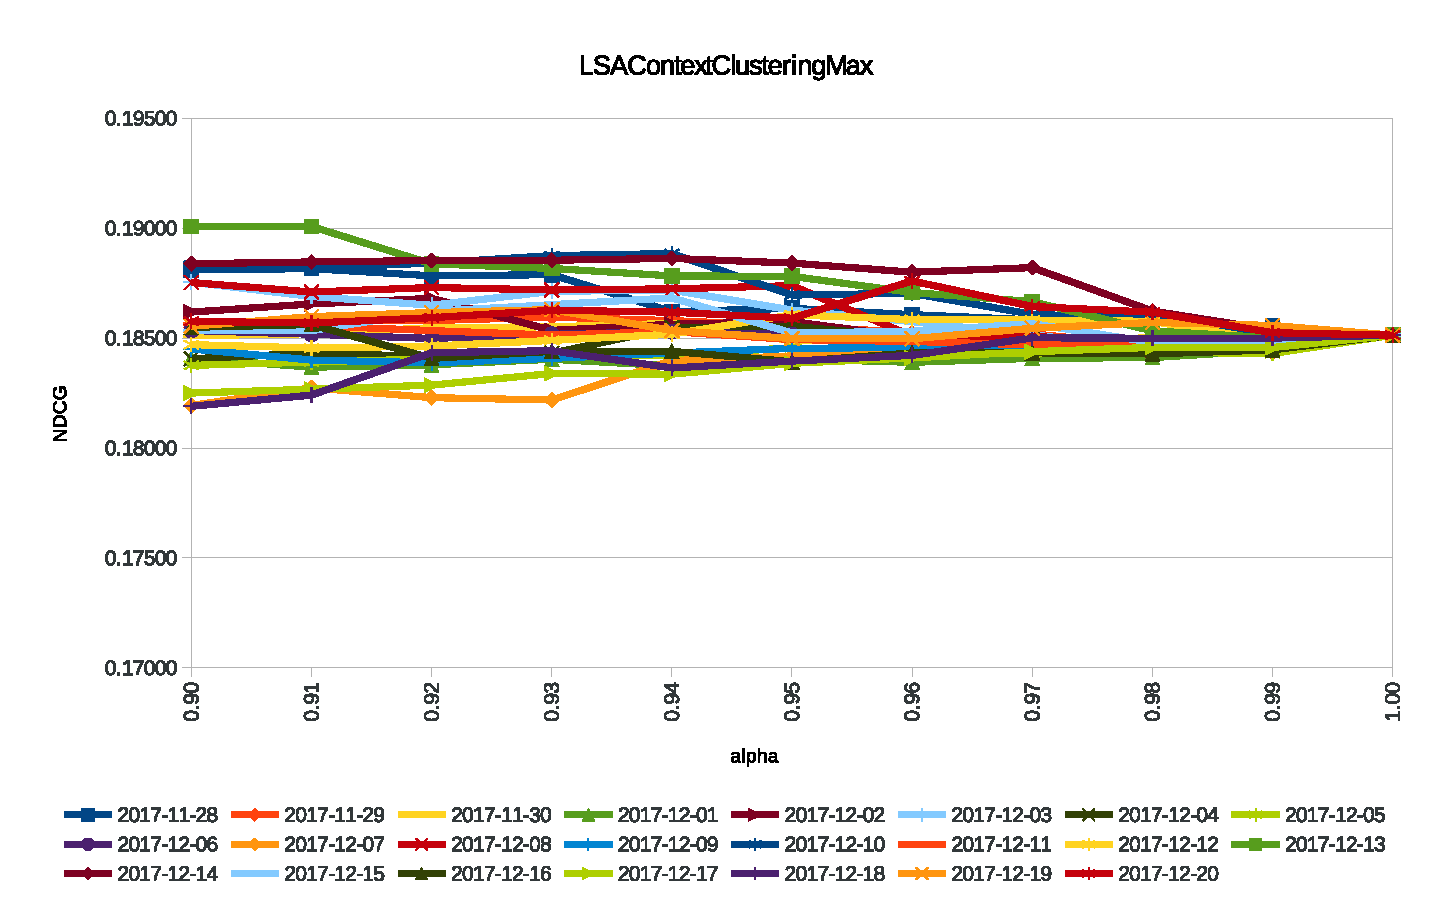
\includegraphics[width=0.33\textwidth]{figures/ndcg-results-proposal-context-fuzzy-clustering-max.eps}
    \label{fig:ndcg-results-proposal-context-fuzzy-clustering-max}
    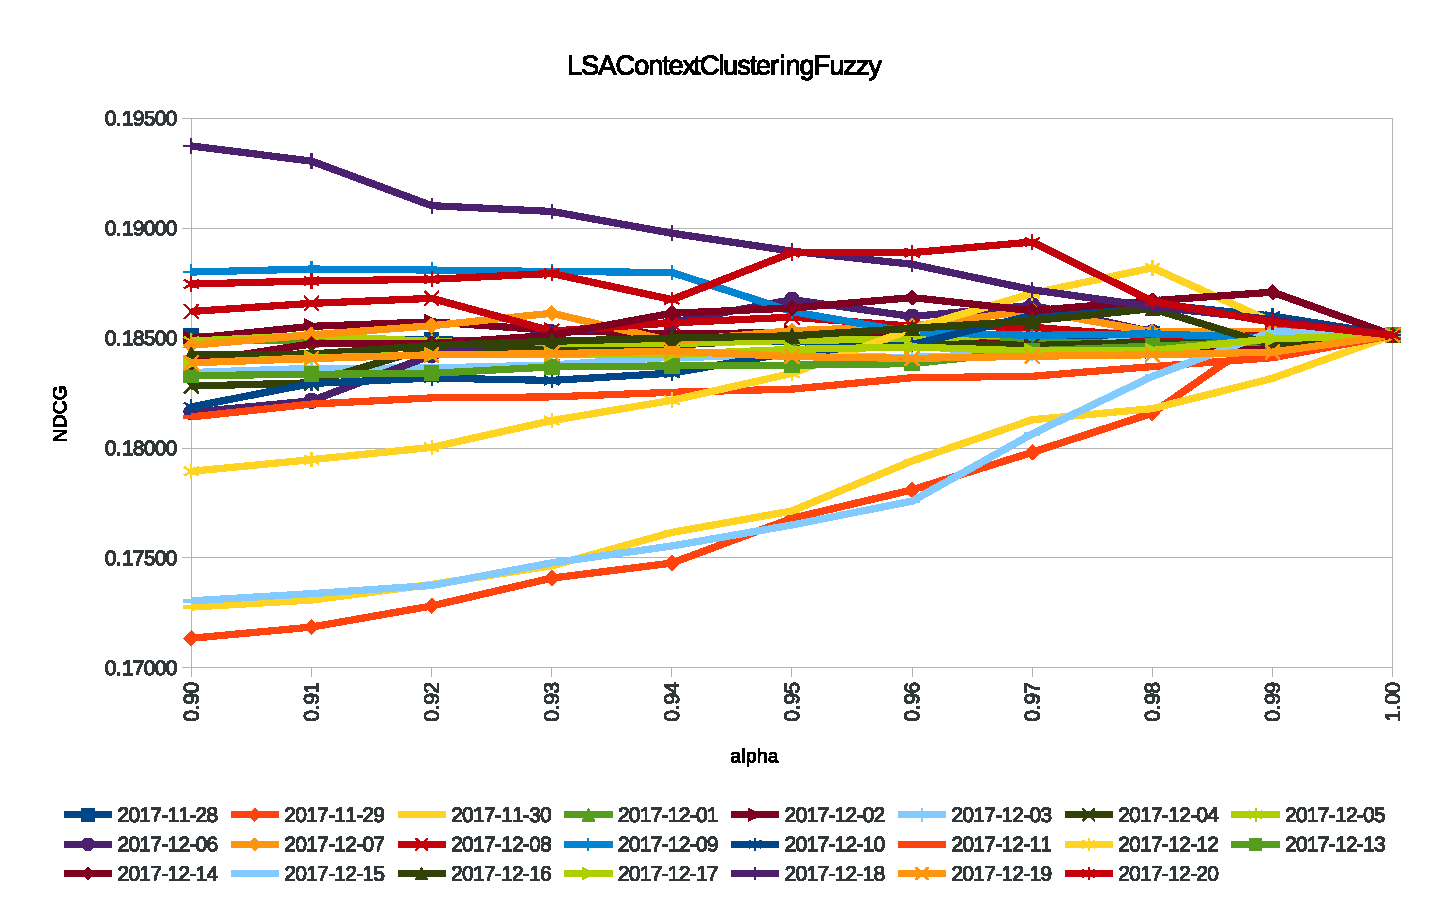
\includegraphics[width=0.33\textwidth]{figures/ndcg-results-proposal-context-fuzzy-clustering-membership.eps}
    \caption{Contextual dataset used in the experiment, where each day has a different status count.}
    \label{fig:ndcg-results-proposal-context-fuzzy-clustering-membership}
\end{figure}

Figures \ref{fig:ndcg-results-proposal-context-no-clustering}, \ref{fig:ndcg-results-proposal-context-fuzzy-clustering-max} and \ref{fig:ndcg-results-proposal-context-fuzzy-clustering-membership} show the results of the 3 techniques compared in the 3dprinting QA dataset. The three figures have the same scale and, in X axis, alpha parameter is shown. The series denote the context, hence its position show the results of the proposal with the correspongding alpha value for the day.

In Figure \ref{fig:ndcg-results-proposal-context-no-clustering} it can be noticed that, alghout the proposal improves the results of LSA in some days (contexts), the improvement does not compensates for the decay in performance in other days. Focusing in the context of 2017-11-28, LSAContext improves the results of LSA for all alpha values.

Figure \ref{fig:ndcg-results-proposal-context-fuzzy-clustering-membership} shows that LSAContextFuzzy improves the results of LSA. It obtains better results than LSAContext, given that the results are distributed more upper than those of the LSAContext aproach. If we focus on the results on single days, it can be noticed that LSAContextFuzzy improves greatly for the context of day 2017-11-28. However, there is a major decay in three contexts: 2017-11-29, 2017-11-30 and 2017-12-15 in which the proposal does not reaches the value of the LSA approach. If we focus specifically on the day 2017-12-12, there is a decay for $\alpha \in [0.90,0.95]$ but it improves the results of LSA for $\alpha \in [0.96,0.99]$.

Figure \ref{fig:ndcg-resutls-proposal-context-fuzzy-clustering-max} shows that LSAContextClustering improves the results of LSA for most of the contexts explored. It consistenly obtains better results than LSA, althought the improvements.

Figure \ref{fig:ndcg-results-3proposals-average} sumarises the results of the three proposals as compared to the LSA approach. It shows that LSAContextFuzzy and LSAContext, although they obtain better results than LSA in some contexts, in average they do not provide improvement. In the case of LSAContextClustering, it overcomes the results of all the remaining approaches for $\alpha \in [0.90,0.97]$. For $\alpha=0.94$ it reached the maximum average NDCG across all contexts explored, hence this value is the best one in this QA domain.

\begin{figure}[htb]
    \centering
    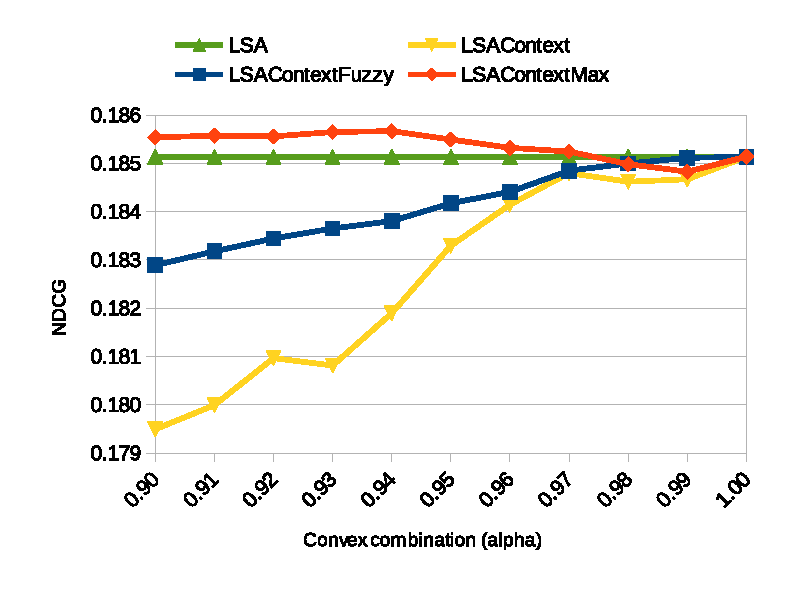
\includegraphics[width=0.33\textwidth]{figures/ndcg-results-3proposals-average.eps}
    \caption{Average NDCG of the compared approaches in all contexts.}
    \label{fig:ndcg-results-3proposals-average}
\end{figure}

The best approaches of the compared ones is the LSAContextClustering with $\alpha=0.94$. This value has been optimised for the 3dprinting QA dataset, hence, for other domains it needs to be adjusted. This parameter provides the LSAContextClustering with flexibility to adapt to different QA domains.

\section{Conclusions}

In this paper, we have explored the application of contextual information in the QA domain recommendation. LSAContextClustering first builds the LSA model associated to the QA domain. After that, it builds the user profile combining the QA profiles with the user preferences. In parallel, it builds the profiles of the context, which is separated in a number of clusters and a context profile is built for each of them. The following step is to combine the user profile with the context profile that is more close to their preferences, which is achieved computing the cosineCoefficient between the profiles. This combined profile allows the system to know user preferences and also consider contextual information in the recommendation. 

We performed a case study to compare various configurations for the proposed approach. It shows that all improvements done provide better results as compared to the baseline method (LSA). We found out that the best way to generate each context cluster profile is to select only the words whose membership value is the highest across clusters in the explored QA domain.

In this scenario, contextual information is a key source of information to provide users with relevant recommendations that allow them to better understand the current scenario. The provided system is a relevant tool in the completion of user knowledge through the recommendation of QA items.

\textbf{\textit{Acknowledgements:}} This research work was partially supported by the Research Project TIN-2015-66524-P, the Spanish FPU fellowship (FPU13/01151).

\section*{Bibliography}
\bibliography{rs-bibliography}

\end{spacing}

\end{document}